\section{Background and Related Work}
\label{sec:background}
For a single attention head, let $Q$, $K$, and $V$ contain $N$ token vectors of dimension $d$. Ignoring masking for the moment, scaled dot-product attention is
\begin{equation}
 O=\operatorname{softmax}(QK^{\mathsf T}/\sqrt{d})V.
 \label{eq:attention}
\end{equation}
The expression specifies the desired result, not the storage policy. A materialized schedule can form a score matrix, normalize it, and then multiply by the values. A tiled schedule can process smaller regions while maintaining the information needed to combine their contributions. The conceptual difference is the lifetime of intermediate data, not a change to the definition in Equation~\ref{eq:attention}.

\subsection{Exactness, scheduling, and numerical behavior}
FlashAttention studies exact attention through an IO-aware tiled algorithm that reduces transfers between GPU memory levels~\cite{dao2022flashattention}. FlashAttention-2 further examines work partitioning and parallelism~\cite{dao2023flashattention2}. We use these works to motivate two distinct concerns: reducing bytes moved and using the available arithmetic resources effectively. We do not copy their performance numbers into the synthetic dataset, and our two abstract schedules are not faithful simulators of either implementation.

Mathematical exactness also needs careful wording. Reordering finite-precision operations may change rounding even when an algorithm evaluates the same mathematical expression. A real correctness study should state the reference precision, tolerated error, and distributions of tested inputs. The absence of an approximation in the mathematical formulation does not remove the need for numerical validation. This paper models time and storage only; it makes no numerical-accuracy claim about executable attention code.

\subsection{Training, prefill, and decoding}
Attention appears in different execution regimes. A full sequence computation exposes a different shape from generating one token while reading a growing cache. Likewise, backward computation has different intermediate requirements from forward-only execution. Our main model describes a simplified forward full-sequence workload. It should not be read as a model of autoregressive decoding, complete training steps, or a production serving system.

PagedAttention addresses key--value cache management and sharing in language-model serving~\cite{kwon2023pagedattention}. Its context helps explain why an attention microbenchmark is not a serving benchmark. A service must also manage admission, batching, memory fragmentation, and request completion. A schedule that improves one dense attention operation can leave those system-level constraints unchanged. Conversely, better cache management can improve useful concurrency without changing the arithmetic expression for an individual head.

\subsection{Three quantities that should not be conflated}
Traffic is the amount of data transferred over a specified boundary during execution. Workspace is the maximum temporary storage simultaneously allocated under a stated lifetime model. Runtime is the duration of an operation under a measurement boundary. A tensor may be allocated once and read many times, so traffic can substantially exceed allocation size. A reduction in workspace may permit a larger batch, but the resulting throughput improvement depends on scheduling and the rest of the model.

We keep these quantities separate in both the notation and the artifact. Traffic expressions use bytes transferred; workspace curves use bytes resident; time curves use seconds. The units are converted only at plot boundaries, with binary units for workspace and decimal units for bandwidth. This bookkeeping is mundane but necessary: an unexplained factor of two can be a unit conversion, a second materialized tensor, or a genuinely different algorithm. Figure~\ref{fig:schedule} summarizes the abstraction used throughout the manuscript.

\begin{figure*}[t]
 \centering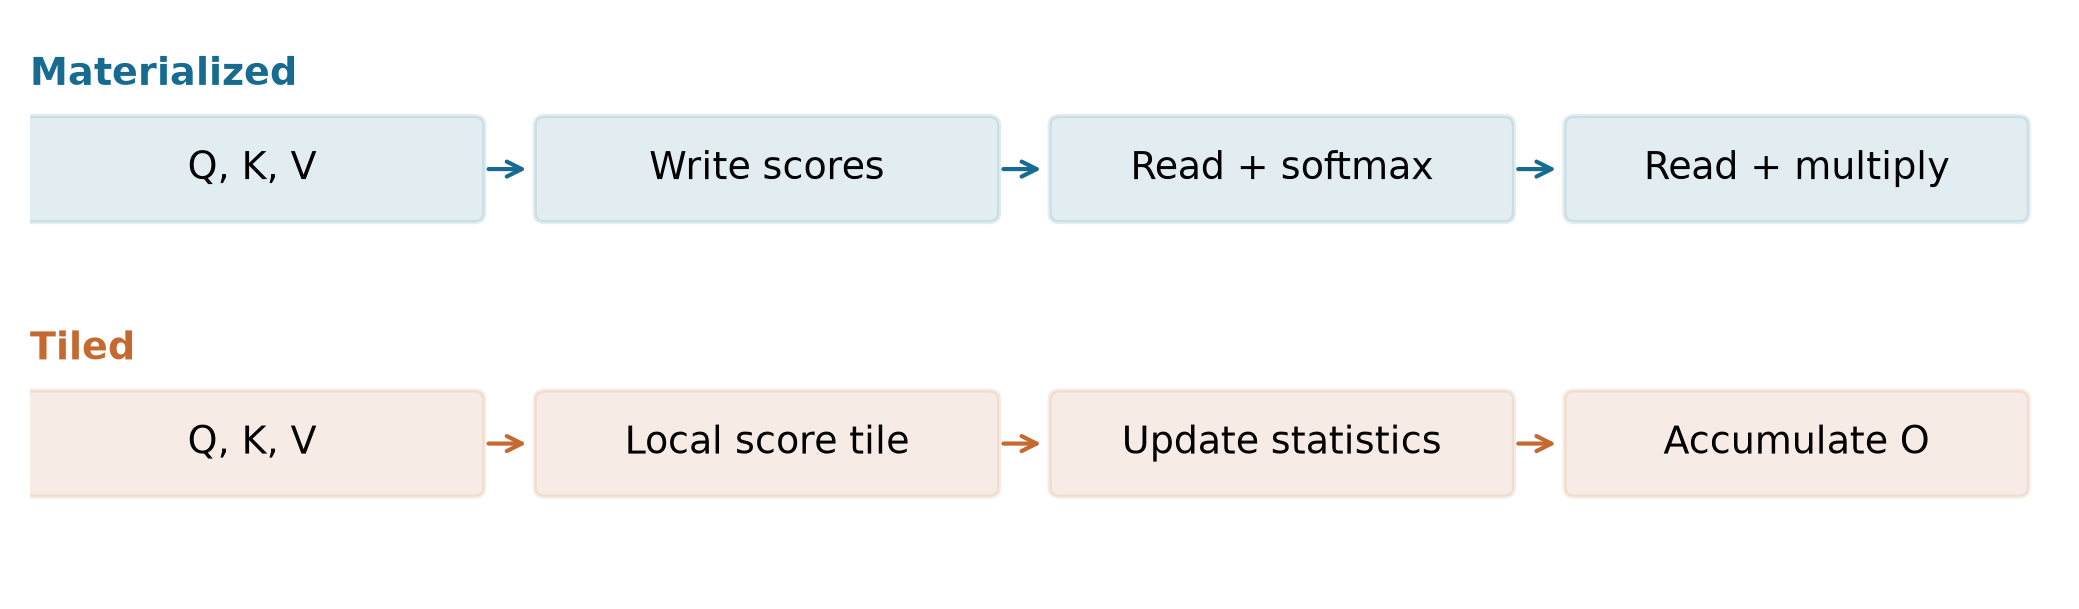
\includegraphics[width=.94\textwidth]{assets/schedule.png}
 \caption{Abstract schedules used in the demonstration. These diagrams explain intermediate lifetimes; they are not GPU implementation traces. Both schedules target the same mathematical attention expression.}
 \label{fig:schedule}
\end{figure*}
